
\documentclass{beamer}

\usepackage{framed}
\usepackage{graphicx}

\begin{document}
\section{Visualizing linear relationships}
%=========================================%
\begin{frame}
	\begin{itemize}
		\item
		Many datasets contain multiple quantitative variables, and the goal of an analysis is often to relate those variables to each other. \item We previously discussed functions that can accomplish this by showing the joint distribution of two variables. It can be very helpful, though, to use statistical models to estimate a simple relationship between two noisy sets of observations. \item The functions discussed in this chapter will do so through the common framework of linear regression.
		\end{itemize}
\end{frame}
%=========================================%
\begin{frame}
	\begin{itemize}
\item In the spirit of Tukey, the regression plots in seaborn are primarily intended to add a visual guide that helps to emphasize patterns in a dataset during exploratory data analyses. 
\item That is to say that seaborn is not itself a package for statistical analysis. To obtain quantitative measures related to the fit of regression models, you should use statsmodels. 
\item The goal of seaborn, however, is to make exploring a dataset through visualization quick and easy, as doing so is just as (if not more) important than exploring a dataset through tables of statistics.
	\end{itemize}

\end{frame}
%=========================================%
\begin{frame}[fragile]
	\begin{verbatim}
%matplotlib inline
import numpy as np
import pandas as pd
import matplotlib as mpl
import matplotlib.pyplot as plt
import seaborn as sns
sns.set(color_codes=True)
np.random.seed(sum(map(ord, "regression")))
tips = sns.load_dataset("tips")
	\end{verbatim}

\end{frame}
%========================================================%
\subsection{Functions to draw linear regression models}
Two main functions in seaborn are used to visualize a linear relationship as determined through regression. These functions, regplot() and lmplot() are closely related, and share much of their core functionality. It is important to understand the ways they differ, however, so that you can quickly choose the correct tool for particular job.
\end{frame}
%===================================================================== %
\begin{frame}[fragile]
	\frametitle{Seaborn Workshop}
	\large
In the simplest invocation, both functions draw a scatterplot of two variables, x and y, and then fit the regression model y ~ x and plot the resulting regression line and a 95\% confidence interval for that regression:
\end{frame}
%===================================================================== %
\begin{frame}[fragile]
	\frametitle{Seaborn Workshop}
	\large
\begin{verbatim}
sns.regplot(x="total_bill", y="tip", data=tips);
\end{verbatim}

\begin{figure}
	\centering
	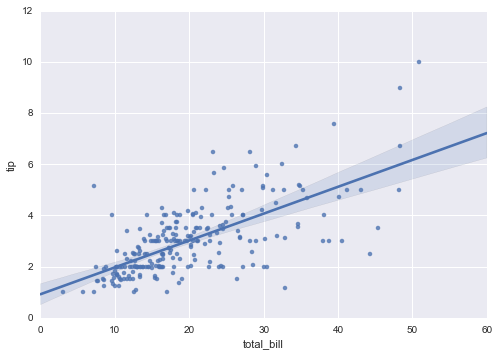
\includegraphics[width=0.7\linewidth]{images/regression_9_0}
\end{figure}
\end{frame}
%===================================================================== %
\begin{frame}[fragile]
	\frametitle{Seaborn Workshop}
	\large
\begin{verbatim}
sns.lmplot(x="total_bill", y="tip", data=tips);
\end{verbatim}
\begin{figure}
	\centering
	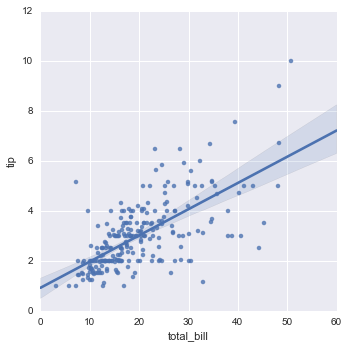
\includegraphics[width=0.7\linewidth]{images/regression_10_0}
\end{figure}
\end{frame}
%===================================================================== %
\begin{frame}[fragile]
	\frametitle{Seaborn Workshop}
	\large
You should note that the resulting plots are identical, except that the figure shapes are different. We will explain why this is shortly. For now, the other main difference to know about is that regplot() accepts the x and y variables in a variety of formats including simple numpy arrays, pandas Series objects, or as references to variables in a pandas DataFrame object passed to data. In contrast, \texttt{lmplot()} has data as a required parameter and the x and y variables must be specified as strings. 

\end{frame}
%===================================================================== %
\begin{frame}[fragile]
	\large
	
\begin{itemize}
\item This data format is called “long-form” or “tidy” data. Other than this input flexibility, \texttt{regplot()} possesses a subset of lmplot()‘s features, so we will demonstrate them using the latter.

\item It’s possible to fit a linear regression when one of the variables takes discrete values, however, the simple scatterplot produced by this kind of dataset is often not optimal:
\end{itemize}
\end{frame}
%===================================================================== %
\begin{frame}[fragile]
	\large
	
sns.lmplot(x="size", y="tip", data=tips);
\begin{figure}
	\centering
	\includegraphics[width=0.7\linewidth]{images/regression_12_0}
\end{figure}
\end{frame}
%===================================================================== %
\begin{frame}[fragile]
	\large
One option is to add some random noise (“jitter”) to the discrete values to make the distribution of those values more clear. Note that jitter is applied only to the scatterplot data and does not influence the regression line fit itself:
\begin{framed}
\begin{verbatim}
sns.lmplot(x="size", y="tip", data=tips, x_jitter=.05);
\end{verbatim}
\end{framed}/
\begin{figure}
\centering
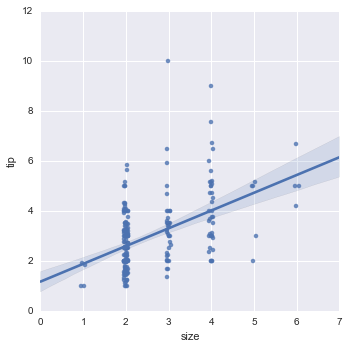
\includegraphics[width=0.7\linewidth]{images/regression_14_0}
\end{figure}


\end{frame}
%===================================================================== %
\begin{frame}[fragile]
	\large
A second option is to collapse over the observations in each discrete bin to plot an estimate of central tendency along with a confidence interval:
\begin{verbatim}
sns.lmplot(x="size", y="tip", data=tips, x_estimator=np.mean);
\end{verbatim}

\begin{figure}
\centering
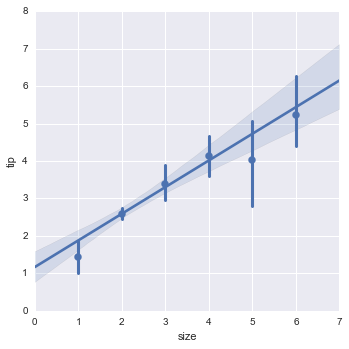
\includegraphics[width=0.7\linewidth]{images/regression_16_0}
\caption{}
\label{fig:regression_16_0}
\end{figure}


\end{frame}
\end{document}